\section{字符串}
现在我们来看一种特殊类型的一维数组:字符串。字符串也是一大类,不过它们的道理很相似,所以我们只研究其中一个部分:\lstinline@char@ 数组。\par
定义一个 \lstinline@char@ 数组的方法和定义一般的一维数组差不多:
\begin{lstlisting}
    char str1[5] = {'J','a','c','k','\0'}; //正常格式,注意末尾最好用'\0'
    char str2[10] {'A','m','y'}; //省略部分内容,省略的部分使用默认值('\0')
    char str3[] {65, 66, 67, '\0'}; //除非末尾用'\0',否则不建议这么写!
\end{lstlisting}
唯一的例外是,我们可以用字符串字面量来初始化字符数组。
\begin{lstlisting}
    char str4[5] {"Jack"}; //效果等同于上述str1的定义
\end{lstlisting}
这是一种语法糖\footnote{语法糖(Syntactic sugar),是指某种编程语言中的某些语法,它们对语言本身的功能没有影响,但是更方便程序员使用。语法糖可以让程序更简洁,有更高的可读性。},实际上编译器会把它解释成和 \lstinline@str1@相同的初始化方式。不过呢,这种针对于字符数组的语法糖让我们初始化内容变得更简单了。然而,这种语法糖仅在初始化时有效。到了赋值的时候,我们不能这样写:
\begin{lstlisting}
    str1 = "Bob"; //错误!
\end{lstlisting}
要想改变字符串的内容,我们只能通过给每个元素赋值的方式来进行:
\begin{lstlisting}
    str1[0] = 'B';
    str1[1] = 'o';
    str1[2] = 'b';
    str1[3] = 0; //不要忘记!
\end{lstlisting}
但是这种逐个赋值的操作可能出问题,我们很容易漏掉 \lstinline@str1[3]=0@ 这句。所以我们推荐使用 \lstinline@cstring@ 库中的函数 \lstinline@strcpy@ 来实现。我们暂时先不讲这个,留到后面再说。
\begin{lstlisting}
    strcpy(str1, "Bob"); //正确
\end{lstlisting}\par
字符串的使用和其它类型的数组很相似,但又有它的特点。所以我们在这里先来介绍一下关于字符串的最基本概念。
\subsection*{字符串是什么?}
我们最熟悉的字符串就是我们一直在使用,但是尚未讲解过的字符串字面量。很多时候我们都要输出字符串字面量。
\begin{lstlisting}
    cout << "Hello World!";
\end{lstlisting}
这里的 \lstinline@"Hello World!"@ 就是一个字符串字面量。\par
字符串字面量不同于基本数据类型的字面量,它是一个数组,我们可以像其它数组名那样去输出它的地址。但是当我们用 \lstinline@cout@ 输出一个字符串字面量的时候,它输出的并不是地址,而是这个字符串的内容啊!\par
类似的问题,我们在指针中也遇到过。当我们试图输出一个指针的时候,实际输出的可能是任何东西,但是怎么看都不像个地址值。这是因为,\lstinline@<<@ 对于 \lstinline@ostream@ 和 \lstinline@const char*@ 类型有特殊的重载。在遇到 \lstinline@char*@ 及其变体的类型时,会把它按照字符串的方式来输出,而不是输出它的地址。\par
为了看到它的地址,我们可以通过显式类型转换,把 \lstinline@char*@ 类型转换成 \lstinline@void*@ 类型然后输出,这样就能看到地址值了。
\begin{lstlisting}
    cout << (void*)"Hello World!"; //输出0x4006a4
\end{lstlisting}
字符串字面量存储在数据段(Data section),这里的内容都是常量,所以字符串是一个常量 \lstinline@char@ 数组。我们可以用 \lstinline@typeid@ 检验。\footnote{MSVC中能看出它是 \lstinline@char const [13]@ 类型,但GCC中只有 \lstinline@A13_c@,看不出常量性,只能知道它是一个 \lstinline@char@ 数组。\lstinline@is_same@ 的检测相对更细致,不过它也有它的问题,见下文。}
\begin{lstlisting}
    cout << typeid("Hello World!").name(); //输出A13_c
\end{lstlisting}
或者是用 \lstinline@is_same@ 检验。但是这里出现了新问题,我们直接写成下面这样是行不通的:
\begin{lstlisting}
    cout << is_same<decltype("Hello World!"), const char[13]>::value;
    //输出0,怎么回事?
\end{lstlisting}
具体的情况比较复杂,这涉及到 \lstinline@decltype@ 的问题\footnote{按标准,\lstinline@decltype("Hello World!")@ 返回的类型是一个对 \lstinline@const char[13]@ 的左值引用类型。},读者不必深究。我们只需改成这样就好:
\begin{lstlisting}
    cout << is_same<decltype("Hello World!"), const char(&)[13]>::value;
    //输出1
\end{lstlisting}
那么既然字符字面量是一个字符数组,我们岂不是可以用下标运算符来访问它的某一个元素?
\begin{lstlisting}
    cout << "Hello World!"[0]; //将输出H
\end{lstlisting}\par
\subsection*{字符串是如何构成的?}
细心的读者可能会发现另一个问题:这个 \lstinline@"Hello World!"@ 带空格和标点也只有12个字符,为什么它的长度是13?这就不得不提到字符串的构成了。\par
在C/C++中,所有的字符串都应当以 \lstinline@'\0'@,也就是ASCII码值为 \lstinline@0@ 的字符结尾。这是我们判断一个字符串有效信息长度的最佳标准。为什么这么说呢?\par
当我们定义字符串时,因为我们也不确定它的有效信息有多长,所以我们可能要给它比较大的容量。
\begin{lstlisting}
    char name[33]; //难免会有名字很长的人,所以容量要大一点
\end{lstlisting}
但是这里就会存在一个问题:绝大部分情况下,这个字符串真实存储的信息长度肯定很少,比如说``Amy Smith'',这个名字只有9个字符,那么我们就还需要一个类似于 \lstinline@size@ 的变量,来说明 \lstinline@name@ 的有效信息长度。问题在于,这个方法比较浪费空间,我们还需要另外定义变量来存储它的长度;而且也很不方便使用,我们每次传参都要额外加一个变量。\par
C/C++有更好的解决方法,那就是用 \lstinline@name@ 数组内的信息来表示有效长度!具体的方法是,我们在有效信息的末尾,把下一个字符设置成 \lstinline@'\0'@。这样,无论哪个函数拿到了这个字符串,它只需要从 \lstinline@name[0]@ 开始数一数,看数到哪里 \lstinline@name[i]=='\0'@,那么自然就知道了这个字符串的长度,而不需要用另外的参数来记录了。\par
举个例子,现在我记录一个名字 \lstinline@"Alexander Alexandrovich Stepanov"@。这个名字碰巧有32个字符(含空格),加上末尾的结束符共有33个。现在我们把它存入 \lstinline@name@ 中。
\begin{lstlisting}
    char name[33] {"Alexander Alexandrovich Stepanov"};
\end{lstlisting}
这时它的33个字节全部都是有效信息,如图5.13第一行所示。\par
\begin{figure}[htbp]
    \centering
    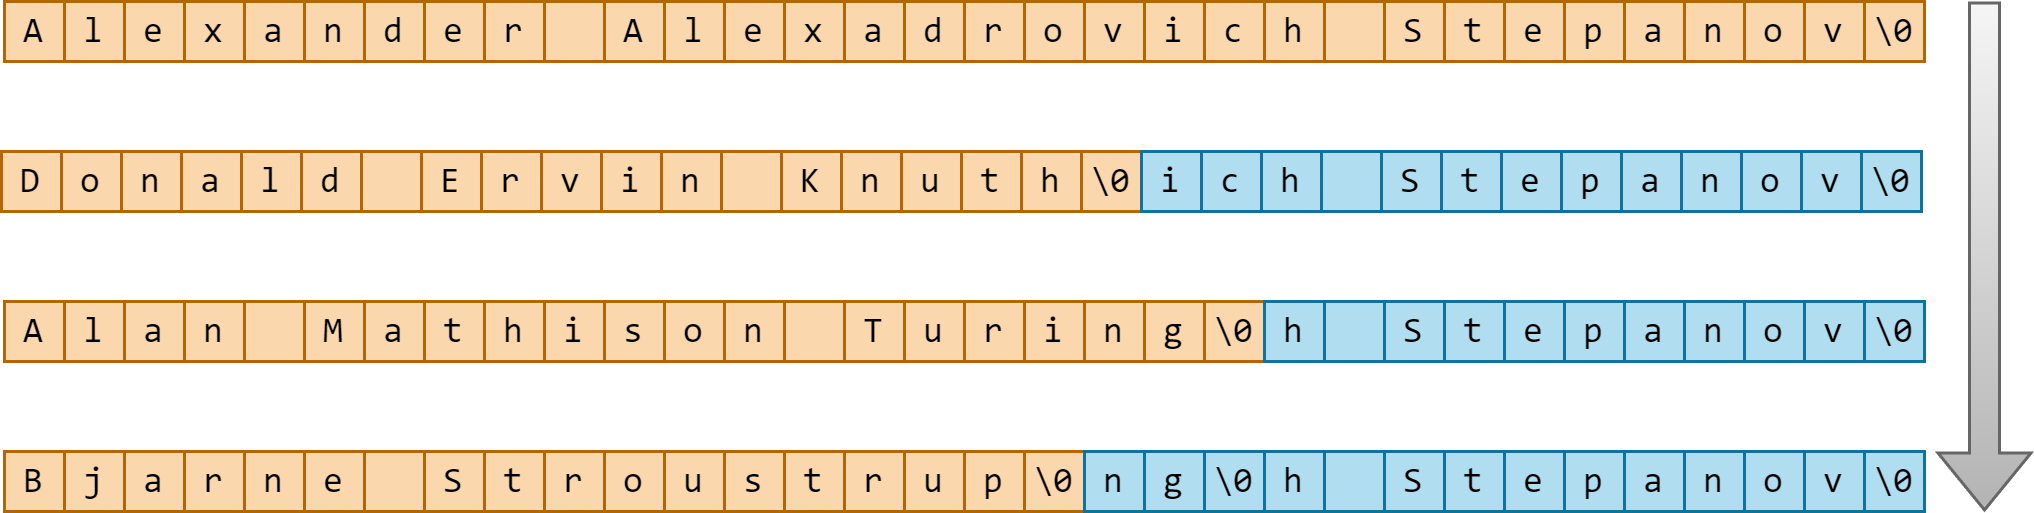
\includegraphics[width=\textwidth]{../images/generalized_parts/05_Information_in_the_string_300.png}
    \caption{字符串 \lstinline@name@ 中信息的变化情况}
\end{figure}
那么接下来我通过 \lstinline@strcpy@\footnote{MSVC会默认阻止我们使用 \lstinline@strcpy@ 和 \lstinline@strncpy@ 函数。为了解决这个问题,我们可以更改设置,或直接在源代码的最前面加一行 \texttt{\#define \_CRT\_SECURE\_NO\_WARNINGS 1}。}把另一个名字复制到 \lstinline@name@ 中,这样做会修改原来字符串的信息。
\begin{lstlisting}
    strcpy(name, "Donald Ervin Knuth");
    //strcpy会把第二个参数中的有效部分复制到第一个参数起的内存空间中
\end{lstlisting}
现在 \lstinline@name@ 的内存空间应该如同图5.13第二行所示。注意,只有第一个 \lstinline@'\0'@ 及以前的部分是有效信息(橙色),而后面的部分不是有效信息(蓝色),我们也没有浪费时间去修改它的必要,让它们维持原状就好。\par
接下来我再次通过 \lstinline@strcpy@ 把另一个名字复制到 \lstinline@name@ 中。
\begin{lstlisting}
    strcpy(name, "Alan Mathison Turing");
    //strcpy会把第二个参数中的有效部分复制到第一个参数起的内存空间中
\end{lstlisting}
现在 \lstinline@name@ 的内存空间应该如同图5.13第三行所示。下一步我再修改 \lstinline@name@ 的值,就应该得到图5.14第四行的情况了。
\begin{lstlisting}
    strcpy(name, "Bjarne Stroustrup");
\end{lstlisting}\par
这就是字符串的基本结构。如果简单点说就是,字符串总是要有一个 \lstinline@'\0'@ 结束符。那么如果我们要输入一个长度为 \lstinline@n@ 的字符串,考虑到末尾结束符的存在,我们就至少需要容量有 \lstinline@n+1@ 的字符串才行。\par
了解了这些之后,我们就可以自己写一些简单的字符串处理函数了。\par
\subsection*{字符串的处理}
知道了字符串的结构之后,我们就可以写一些简单的函数来进行字符串的处理了。\par
\lstinline@cstring@ 库中有一些常见的字符串处理函数——有些我们也可以写,比如 \lstinline@strlen@。这个函数可以计算一个字符串有效信息的长度(不包含结束符)。比如说,\lstinline@sizeof("Amy")@ 得到 \lstinline@4@,这是它占用内存的大小;而 \lstinline@strlen("Amy")@ 得到 \lstinline@3@ 这是它外表展现出来的长度。\par
为了避免名字冲突,我们就写一个 \lstinline@StrLen@ 函数,它可以接收 \lstinline@char@ 指针\footnote{一般来说,我们在涉及其它类型的数组参数时会使用数组形式的形参,以便告诉用户它接收的是数组(虽然实际情况还是转换成指针了)信息;而在涉及字符串时,我们更习惯于把参数设为指针类型。},并返回一个无符号的整数,作为长度。\par
来考虑一下这个函数的外在特征。我们只需提供这个字符串就可以了,无需更多信息。不过我们只想求值,不需要改变它,所以干脆设成指向常量的指针,稳妥一些。至于返回值,\lstinline@strlen@ 内部使用的是 \lstinline@size_t@ 类型作为返回值,其实我们用 \lstinline@unsigned@ 或者 \lstinline@unsigned long long@ 也行。\par
\begin{lstlisting}
unsigned StrLen(const char*); //声明完毕
\end{lstlisting}\par
接下来考虑怎么求出它的长度。其实很简单,我们从 \lstinline@str@ 指向的第一个字符开始找,直到找到 \lstinline@'\0'@ 为止,走过了多少个字符,就说明它的长度是多少啦。所以我们可以用一个循环结构来实现这个功能。
\begin{lstlisting}
unsigned StrLen(const char* str) {
    for (unsigned i = 0; ; i++) { //条件留空将默认为true
        if (str[i] == '\0') //如果str[i]==0,说明字符串结束了
            return i; //直接返回i的值
    }
}
\end{lstlisting}\par
写完了之后一定不要得意忘形,马上在主函数中写一个例子验证一下,看看是否合乎我们的预期。比如 \lstinline@StrLen("Amy")@,它的值就应该是 \lstinline@3@,我们可以输出一下看看对不对。\par
接下来我们再写一个稍难的函数。\lstinline@strcpy@ 函数可以把一串内容复制到另一个字符串中,效果等同于``字符串间的赋值'',这样可以免于让我们用逐个字符赋值的麻烦方法来改变整个字符串的值。它接收两个参数,第一个参数 \lstinline@dest@ 是目标字符串,第二个参数 \lstinline@src@ 是内容源。这个函数不需要考虑 \lstinline@dest@ 的容量是否足够,只管往里复制就行\footnote{实际上,它也没办法顾及 \lstinline@dest@ 的容量够不够,因为字符串作为数组类型,在传递参数时就会变成指针类型,在此过程中它的长度信息就已经丧失了,除非我们人为地把长度信息也传入其中。}。\par
换句话说,我们只需要把 \lstinline@src@ 串中的有效部分逐个赋值给 \lstinline@dest@ 的对应部分就行。比如说,\lstinline@dest[0]=src[0]@,然后 \lstinline@dest[1]=src[1]@,诸如此类。终止条件是 \lstinline@src[i]=='\0'@,这时我们就可以停止了。但是最后不要忘了人为地在后面补上一个 \lstinline@'\0'@ 结束符,否则这个字符串就就没有结束。\par
所以我们就来模仿赋值语句的方式来写一个 \lstinline@StrCpy@ 函数。它的第一个参数是 \lstinline@char*@ 类型的,第二个参数是 \lstinline@const char*@ 类型的(因为不需要修改,那么就从定义层面防止修改),而返回值是 \lstinline@char*@ 类型的,它的值(地址)应该等于第一个参数的值(地址),这是为了实现类似于赋值运算符的那种连续赋值语法(\lstinline@StrCpy(str1,StrCpy(str2,str))@)。\par
\begin{lstlisting}
char* StrCpy(char*, const char*);
\end{lstlisting}
定义部分看上去好像很难,但我们分析了一通之后会发现,那也只不过是一种逐个赋值的语法而已,所以用 \lstinline@for@ 循环简单写一写就足够了。
\begin{lstlisting}
char* StrCpy(char *dest, const char *src) {
    for (unsigned i = 0; (dest[i] = src[i]) != '\0'; i++) { ; } //还能这样?
    return dest; //返回dest的值
}
int main() { //主函数
    char str[10] {"AbCdEfG"}; //定义str,并预先用其它内容占据
    cout << StrCpy(str, "Bob"); //如果输出Bob,说明代码正确
    return 0;
}
\end{lstlisting}
读者可以运行一下这段代码。如果不出意外的话,结果会输出 \lstinline@Bob@。\par
这里的 \lstinline@StrCpy@ 的逻辑写的比较有技巧性,我们来拆解一下。在 \lstinline@for@ 循环中,我们先初始化了 \lstinline@i=0@,这是循环的起始条件。接下来,我们进行判断。判断语句 \lstinline@(dest[i]=src[i])!='\0'@ 将会先执行 \lstinline@dest[i]=src[i]@ 这个赋值,其返回值 \lstinline@dest[i]@ 会与 \lstinline@'\0'@ 比较。如果不相等,那就说明没有遇到结束符,循环继续。主体部分只有一个分号(甚至可以什么也没有),它表示什么也不做。既然什么也不做,那就直接运行迭代语句 \lstinline@i++@,进入下一轮循环判断就好。如此,我们也可以省了单独为 \lstinline@dest@ 数组添加一个结束符的麻烦——因为在判断它是不是 \lstinline@'\0'@ 之前,我们就已经做了赋值操作了。\par
\subsection*{字符串的输入}
现在我们再来讲讲字符串是如何输入的。\par
最简单的输入方式莫过于用 \lstinline@cin<<@ 来进行输入。
\begin{lstlisting}
    char str[33];
    cin >> str; //直接用cin向字符串中输入
\end{lstlisting}
但是这样就可能会遇到问题。如果我们要向字符串中输入两个英文名,比如 \lstinline@Bjarne Stroustrup@ 和 \lstinline@Alan Mathison Turing@,我们可能就会遭遇这样的困难:
\begin{lstlisting}
    char name1[33], name2[33]; //定义两个字符串用于输入人名
    cin >> name1 >> name2; //连续输入两个人名
    cout << name1 << endl << name2; //输出第一个人名,再换行,再输出第二个人名
\end{lstlisting}
如果我们真的运行一下,就会发现情况好像不太对劲。\\\noindent\rule{\linewidth}{.2pt}\texttt{
\textbf{Bjarne Stroustrup}\\\textit{(刚按下回车键,准备输入第二个人名,结果程序就开始输出了)}\\
Bjarne\\
Stroustrup
}\\\noindent\rule{\linewidth}{.2pt}
这是怎么回事?\par
这是因为,用 \lstinline@cin<<@ 输入字符串时,它断句的方式是在每个空白字符\footnote{空白字符(Whitespace character),在ASCII字符区内包括 \lstinline@'\\t'@, \lstinline@'\\n'@, \lstinline@'\\v'@, \lstinline@'\\f'@, \lstinline@'\\r'@, \lstinline@' '@。如果要判断某个字符是否是空白字符,可以用 \lstinline@cctype@ 库中的 \lstinline@isspace@ 函数来处理,如 \lstinline@isspace('a')@,返回值是 \lstinline@0@。}处断开。所以在输入 \lstinline@name1@ 时,它只会读取到空格之前的内容,而把 \lstinline@Stroustrup@ 这个输出留给下一个输入,即 \lstinline@name2@。这也就解释了为什么当我们按下回车键的时候它就开始输出了,这是因为程序已经把两个字符串读完,接下来当然就是执行输出了。同时这也是输出 \lstinline@name1@ 时得到 \lstinline@Bjarne@ 而输出 \lstinline@name2@ 时得到 \lstinline@Stroustrup@ 的原因。\par
怎么解决呢?我们可以用 \lstinline@cin@ 的成员函数 \lstinline@get@ 或者是 \lstinline@istream@ 类的成员函数 \lstinline@getline@ 来解决。先来讲讲 \lstinline@getline@。\par
\subsubsection*{\lstinline@getline@ 成员函数}
\lstinline@getline@ 成员函数的定义语法有如下两种,它们是重载关系:
\begin{lstlisting}
istream& getline(char_type *s, streamsize count); //重载1
istream& getline(char_type *s, streamsize count, char_type delim); //重载2
\end{lstlisting}
其中的 \lstinline@s@ 是待输入的字符串,而 \lstinline@count@ 表明这个字符串的容量(不同于 \lstinline@strcpy@,这里必须提供容量参数)。对于第一个重载来说,它的含义就是:读取一整行输入,直到遇到回车符\footnote{回车符会被提取,但不会存入 \lstinline@s@ 字符串中。},才停止输入;或者是 \lstinline@count@ 长度的字符串容纳不了用户输入的内容量,这时输入也会停止,同时 \lstinline@cin@ 会进入``fail''状态(我们需要用 \lstinline@input_clear@ 来恢复 \lstinline@cin@,并清理输入流)。\par
接下来我们可以用 \lstinline@getline@ 来输入一些有空格的名字了。程序不会在空格字符处断句,只会在回车字符处断句。\par
\begin{lstlisting}
    constexpr unsigned NameLen {33}; //把名称字符串容量设为33,便于统一
    char name1[NameLen], name2[NameLen]; //定义两个字符串用于输入人名
    cin.getline(name1, NameLen).getline(name2, NameLen); //getline可以连续使用
    cout << name1 << endl << name2; //输出第一个人名,再换行,再输出第二个人名
\end{lstlisting}
本程序的运行结果是\\\noindent\rule{\linewidth}{.2pt}\texttt{
\textbf{Bjarne Stroustrup\\
Alan Mathison Turing}\\
Bjarne Stroustrup\\
Alan Mathison Turing
}\\\noindent\rule{\linewidth}{.2pt}\\
这就合乎我们的预期了。\par
至于第二种重载,无非就是把分隔符从换行符换成了自定义的字符而已,没什么特别的,这里就不再赘述。\par
\subsubsection*{\lstinline@get@ 成员函数}
\lstinline@istream@ 类的 \lstinline@get@ 成员函数的功能比 \lstinline@getline@ 更丰富。以下是 \lstinline@get@ 函数的一部分重载:
\begin{lstlisting}
int_type get(); //(1)
istream& get(char_type &ch); //(2)
istream& get(char_type *s, streamsize count); //(3)
istream& get(char_type *s, streamsize count, char_type delim); //(4)
\end{lstlisting}
重载(1)和(2)的作用都是读取输入流中的单个字符。我们在 \lstinline@input_clear@ 中就用过(1)。
\begin{lstlisting}
void input_clear(istream &in) { //默认参数cin,已在定义中注明
    in.clear();
    while (in.get() != '\n') //get()的作用读取下一个字符
        continue;
}
\end{lstlisting}
\lstinline@get()@ 的返回值是取读的字符所对应的ASCII值,我们可以拿它与 \lstinline@'\n'@ 作比较。如果不相等,就说明还没有读取到回车符,循环继续;一旦读取到回车符,\lstinline@while@ 循环即终止,函数结束。\par
重载(3)和(4)与 \lstinline@getline@ 十分相似,但它们有着细微的区别,在于如何处理结束符。\lstinline@getline@ 会把结束符一并提取(形象点说,吞掉);而 \lstinline@get@ 不会把结束符一并提取,结束符仍然保留在输入流中,下一个输入还会从这个字符开始。所以这样写就不行:
\begin{lstlisting}
    cin.get(name1, NameLen).get(name2, NameLen); //name1正常,但name2为空
\end{lstlisting}
这是因为,\lstinline@name1@ 输入完成后,\lstinline@get@ 函数遇到回车符但没有吞掉它,回车符仍在输入流中,于是输入 \lstinline@name2@ 的时候,程序第一眼看到 \lstinline@'\n'@ 就把输入给结束了,\lstinline@name2@ 当然就会什么也没有了。\par
为了把输入流中的回车符吞掉,我们可以这样写:
\begin{lstlisting}
    cin.get(name1, NameLen).get(name2[0]).get(name2, NameLen);
    //先用name2[0]吞一下回车符,再输入name2,没影响
\end{lstlisting}\par
或者干脆点,直接用 \lstinline@getline@ 就好。\par
